\documentclass[12pt]{article}

\usepackage{orcidlink} % to insert a hyperlinked ORCiD logo
\usepackage{amssymb}
\usepackage{physics}
%\usepackage{cite}
\usepackage{hyperref} % for hyperlinks in references

\usepackage{caption} % for \caption*

\textwidth 160mm
\textheight 230mm
\voffset = -20mm

%Title of paper
%\title{Integration of the Grand Partition Function Functional}
\title{The Morse potential}

\author{R.V.~Romanik
	\\ \small Institute for Condensed Matter Physics, NAS of Ukraine 
	\\ \small 1~Svientsitskii Street, 79011, Lviv, Ukraine 
	\\ \small romanik@icmp.lviv.ua}
%\author{R.V.~Romanik \\ Institute for Condensed Matter Physics, NAS of Ukraine}

\begin{document}
	
	\maketitle
	
	%\begin{multicols}{2}
	
	\abstract{The Morse potential is considered in general.
		\\	
		\textbf{Keywords: } Simple fluids, Morse potential.
	}
	
	\section{Overview}
	The Morse potential $U_{M}(r)$ is given by
	
	\begin{equation}
		\label{def:morse}
		U_{M}(r) = \varepsilon \boldsymbol{(}\exp{[-2(r-R_0)/\alpha]}-2\exp{[-(r-R_0)/\alpha]}\boldsymbol{)}.
	\end{equation}
	It was first introduced in~\cite{Morse1929} to study the vibration spectrum of diatomic molecules.
	Its minimum is located at 
	\begin{equation}
		r_{\rm min}=R_0,
	\end{equation}
	which is found from the condition
	\begin{equation}
		\frac{\partial U_{M}(r)}{\partial r} = 0,
	\end{equation}
	and the depth of the minimum is $\varepsilon$,
	\begin{equation}
		U_{M}(R_0) = -\varepsilon.
	\end{equation}
	Its zero, $U_M(r) = 0$, is located at 
	\begin{equation}
		\sigma = R_0 - \alpha \ln(2),
	\end{equation}
	so that 
	\begin{equation}
		U_M(\sigma) = 0.
	\end{equation}
	The long-range limit is
	\begin{equation}
		\lim_{r \to \infty} U_M(r) = 0.
	\end{equation}
	The value of $U_M(r)$ at $r=0$ is
	\begin{eqnarray}
		U_M(0) & = & \varepsilon \left[\exp(2R_0/\alpha)-2\exp(R_0/\alpha) \right]
		\\
		& = & \varepsilon {\rm e}^{R_0/\alpha} \left({\rm e}^{R_0/\alpha}-2 \right).
	\end{eqnarray}

	It is natural to select the measure units for energy as $\varepsilon$ and for length as $\sigma$. The Morse potential can now be rewritten as
	\begin{equation}
		U_M(r) = \varepsilon {\rm e}^{R_0/\alpha} \left\{ {\rm e}^{R_0/\alpha} \exp[-2\frac{r}{\sigma}\left(\frac{R_0}{\alpha} - \ln2\right)] - 2\exp[-\frac{r}{\sigma} \left(\frac{R_0}{\alpha} - \ln2\right)] \right\}
	\end{equation}
	where the following equalities are taken into account:
	\begin{equation}
		\frac{R_0}{\sigma} = \frac{R_0/\alpha}{R_0/\alpha - \ln2},
		\quad
		\frac{\alpha}{\sigma} = \frac{1}{R_0/\alpha - \ln2}.
	\end{equation}
	As can be seen from the above expressions, the Morse potential expressed in reduced units is parametrized by only one parameter, $R_0/\alpha$. Figure~\ref{morse_vs_param} shows the dependence of $U_M$ on distance $r$ for a few parameter values $R_0/\alpha$. With increasing $R_0/\alpha$, the range of interaction decreases, or in other words, the potential well becomes narrower.
	
	\begin{figure}[htbp]
		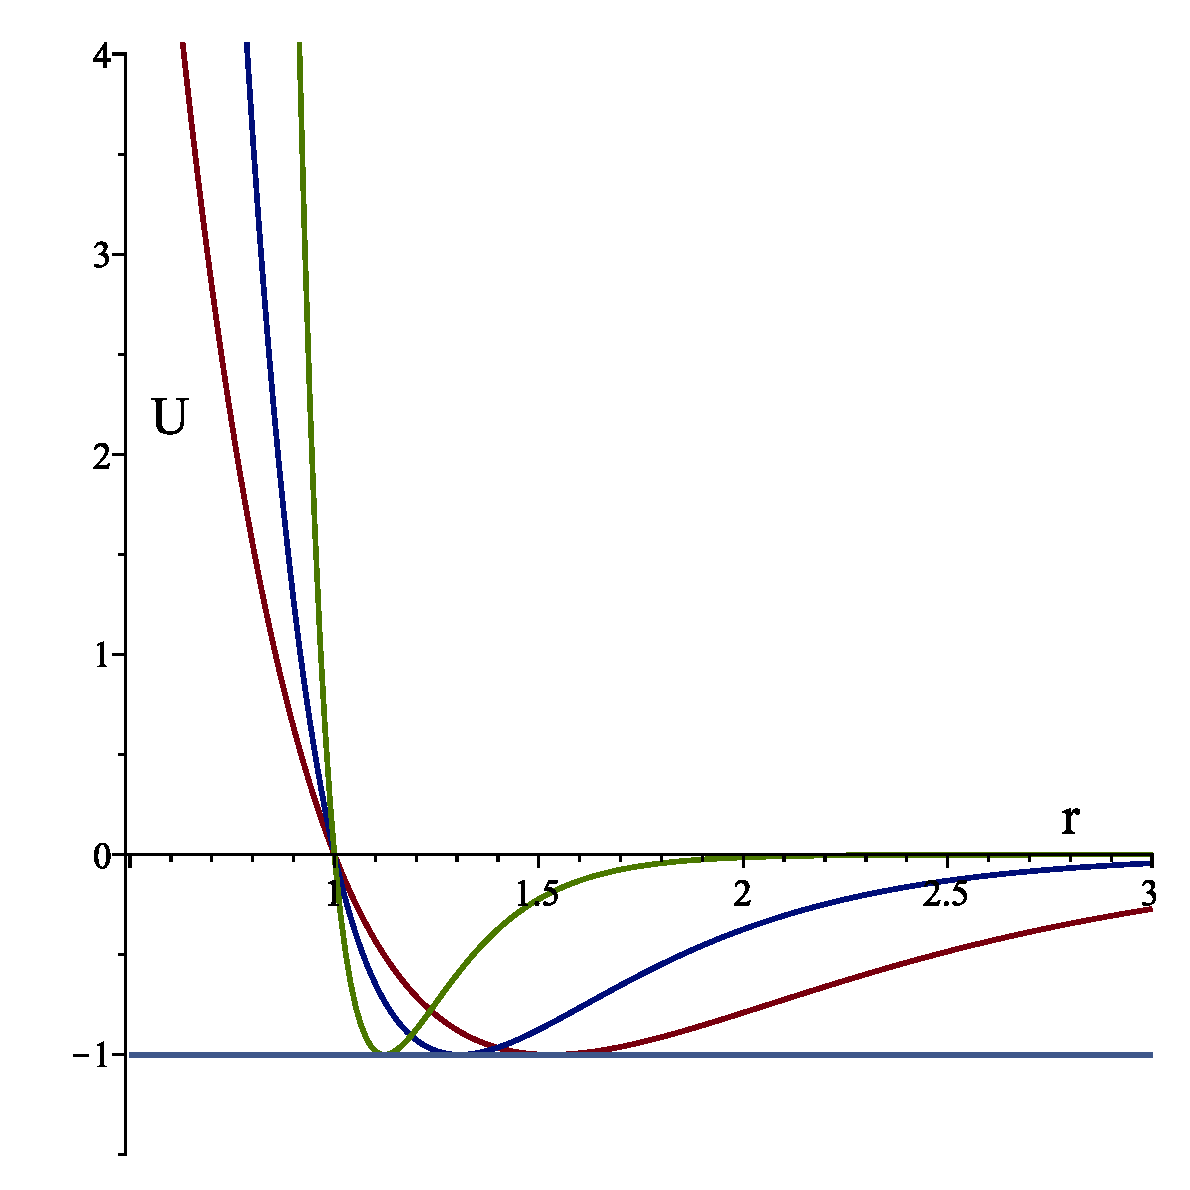
\includegraphics[width=0.7\textwidth, angle=0]{morse_vs_param} 
		{\caption{\label{morse_vs_param} The Morse potential $U_M(r)$ as a function of distance $r$ for a few parameter values. RED - $R_0/\alpha = 2.0$; BLUE - $R_0/\alpha = 2.9544$; GREEN - $R_0/\alpha = 6.35$.
		}}
	\end{figure}
	
	A little bit different form of parametrization, used in~\cite{MartinezValenciaEtAl2013}, is achieved by introducing the following variables:
	\begin{equation}
		r^* = \frac{r}{\sigma}, \quad \beta = \frac{R_0}{\alpha} - \ln2.
	\end{equation}
	In such case, the Morse potential takes on the form as follows:
	\begin{equation}
		U_M(r^*) = 4\varepsilon\left[{\rm e}^{-2\beta(r^* - 1)} - {\rm e}^{-\beta(r^* - 1)}\right].
	\end{equation}
	The minimum is located at
	\begin{equation}
		r^*_{\rm min} = 1 + \beta^{-1} \ln2.
	\end{equation}
	Parameters $R_0$ and $\alpha$ are expressed via $\beta$ as follows:
	\begin{equation}
		\frac{R_0}{\sigma} = 1 + \beta^{-1} \ln2, \quad \frac{\alpha}{\sigma} = \beta^{-1},
	\end{equation}
	and reversely
	\begin{equation}
		\beta = \frac{\sigma}{\alpha} = \frac{\ln2}{\frac{R_0}{\sigma} - 1}.
	\end{equation}
	
	There exist a lot of studies on\ the Morse potential and its application to describing different physical properties of metals. In~\cite{GirifalcoWeizer1959} the potential parameters were presented for the following cubic metals: Pb, Ag, Ni, Cu, Al, Ca, Sr, Mo, W, Cr, Fe, Ba, K, Na, Cs, Rb. In~\cite{LincolnKoliwadGhate1967} the second- and third-order elastic constants were studied, and the Morse potential parameters were presented for the following metals: Al, Cu, Ag, Au, Na, and K. 
	
	The calculation of the vapor-liquid coexistence curve of Morse fluid was performed in the following works: in~\cite{OkumuraYonezawa2000} for such parameters as to compare with the Lennard-Jones potential; in~\cite{SinghAdhikariKwak2006,KwakSinghAdhikari2007} for parameters corresponding to Al, Cu, Au, Na, K; in~\cite{ChengXu2007} with application to Ni; in~\cite{Apfelbaum2011} using an integral-equations approach, with application to Fe.
	
	A recent review on the applications of the Morse potential can be found in~\cite{JacobsonThompson2022}.
	
	\section{Modified Morse potentials}
	The Morse potential with a repulsive term was used in~\cite{MartinezValenciaEtAl2013}
	\begin{equation}
		U(r^*) = \varepsilon\left(\frac{1}{r^*}\right)^{n_p} + 4\varepsilon\left[{\rm e}^{-2\beta(r^* - 1)} - {\rm e}^{-\beta(r^* - 1)}\right],
	\end{equation}
	where $n_p$ took on values between 20 and 70.
	
	A generalized Morse potential was used in works~\cite{BiswasHamann1985, Lim2005}
	\begin{equation}
		\label{def:gen_morse}
		U(r) = A_1 {\rm e}^{-\lambda_1 r} + A_2 {\rm e}^{-\lambda_2 r}.
	\end{equation}
	This generalization increases the number of parameters for the potential. The form~\eqref{def:gen_morse} reduces to the usual form~\eqref{def:morse} with the help of the following substitutions:
	\begin{eqnarray*}
		A_1 = \varepsilon {\rm e}^{2R_0/\alpha}, & & A_2 = -2\varepsilon {\rm e}^{R_0/\alpha}
		\\
		\lambda_1 = 2\alpha^{-1}, & & \lambda_2 = \alpha^{-1}.
	\end{eqnarray*}
	The last equalities can also be obtained by imposing the following restrictions on~\eqref{def:gen_morse}:
	\begin{equation*}
		\varepsilon = \frac{\lambda_1 - \lambda_2}{\lambda_2} A_1 {\rm e}^{-\lambda_1 R_0}
		= \frac{\lambda_2 - \lambda_1}{\lambda_1} A_2 {\rm e}^{-\lambda_2 R_0},		
	\end{equation*}
	\begin{equation}
		\lambda_1 = 2\lambda_2 = 2\alpha^{-1}.
	\end{equation}
	
	
	\bibliographystyle{cmpj}
	\bibliography{fluids_general}
\end{document}